\documentclass[a4paper]{article}
\usepackage[utf8]{inputenc} % Skal passe til editorens indstillinger
\usepackage[english]{babel} % danske overskrifter


\newcommand{\name}{Carsten Nielsen}
%\newcommand{\stnumber}{s123369, s123161, s123821}
\newcommand{\course}{INI 404 Neuromorphic Engineering~I}
\newcommand{\university}{University of Zürich}
\newcommand{\studyline}{Institute of Neuroinformatics}
\newcommand{\assignment}{Lab 8 Post-Lab}
\renewcommand{\date}{\today} %If another date, than that of today is desiered


% Palatino for rm and math | Helvetica for ss | Courier for tt
\usepackage{mathpazo} % math & rm
\linespread{1.05}        % Palatino needs more leading (space between lines)
\usepackage{palatino} % tt
\normalfont
\usepackage[T1]{fontenc}
\usepackage[english]{babel}

\usepackage{graphicx}%allerese hentet % indsættelse af billeder
\usepackage{epstopdf} %Tilfj "--enable-write18" i argumentet for LaTex build. Dette vil konvertere .eps figurer til pdf-format
\graphicspath{{./picture/}} % stivej til bibliotek med figurer
\usepackage{subcaption} %Til gruppering af figurer
\usepackage{amsmath} %matpakke
\usepackage{amsfonts} %
\usepackage{amssymb} %
\usepackage{steinmetz} % flere matematik symboler
\usepackage{polynom} %for displaying polynom division
\usepackage{mathtools} % matematik - understøtter muligheden for at bruge \eqref{}
\usepackage{float}
\usepackage{placeins}
\usepackage{hhline}

%
\usepackage[usenames,dvipsnames]{xcolor}
\usepackage[compact,explicit]{titlesec}% http://ctan.org/pkg/titlesec
%
\usepackage[europeanresistors]{circuitikz}
\usepackage{pgfplots}
\usepgfplotslibrary{patchplots}
\pgfplotsset{compat=1.11}

%---------%
%Easy edit%
%---------%

%Section formating. arg1 is supplied when making section
\newcommand\presectionnumber[1]{~~}
\newcommand\postsectionnumber[1]{}
\newcommand\midlesection[1]{#1}
\newcommand\sectionnum[1]{\arabic{#1}}
\newcommand\subsectionnum[1]{\arabic{#1}}
\newcommand\subsubsectionnum[1]{\alph{#1}}



%------------%
%setion setup%
%------------%
\renewcommand\thesection{Opgave~\sectionnum{section}} %pas p�, kun i matematik
\renewcommand\thesubsection{\thesection,~\subsectionnum{subsection}}
\definecolor{MagRed}{RGB}{190,40,15}
\definecolor{MathGreen}{RGB}{82,164,0}

\titleformat{\section}{\normalfont\sffamily\large\bfseries\color{MathGreen}}{}{0pt}{|\kern-0.15ex|\kern-0.15ex|\kern-0.15ex|\presectionnumber{#1}\sectionnum{section}\postsectionnumber{#1}\qquad\quad\midlesection{#1}\label{sec:\sectionnum{section}}}
\titleformat{\subsection}[runin]{\large\bfseries}{}{10pt}{\sectionnum{section}.\subsectionnum{subsection})~#1\label{sec:\sectionnum{section}.\subsectionnum{subsection}}}
\titleformat{\subsubsection}[runin]{\itshape}{}{0pt}{\subsectionnum{subsection},\subsubsectionnum{subsection}~#1\label{sec:\sectionnum{section}.\subsectionnum{subsection}.\subsubsectionnum{subsubsection}}}
%\titleformat{\subsubsection}{\bfseries}{}{0pt}{\alph{subsection}.\arabic{subsubsection})\qquad\quad#1\label{\arabic{section}\alph{subsection}\arabic{subsubsection}}}

%----------%
%page setup%
%----------%
\textwidth = 400pt
\marginparwidth = 86pt
\hoffset = -25pt
\voffset= -30pt
\textheight = 670pt

%--------%
%hyperref%
%--------%
\newcommand{\HRule}{\rule{\linewidth}{0.5mm}}
\usepackage{fancyhdr}
\usepackage[plainpages=false,pdfpagelabels,pageanchor=false]{hyperref} % aktive links
\hypersetup{%
  pdfauthor={\name},
  pdftitle={\assignment},
  pdfsubject={\course} }
%\usepackage{memhfixc}% rettelser til hyperref

%-------------%
%Headder setup%
%-------------%
\fancyhf{} % tom header/footer
\fancyhfoffset{20pt}
\fancyhfoffset{20pt}
\fancyhead[OL]{\name \\ INI 404}
\fancyhead[OC]{Date \\ \date}
\fancyhead[OR]{\university\\ \studyline}
\fancyfoot[FL]{}
\fancyfoot[FC]{\thepage}
\fancyfoot[FR]{}
\renewcommand{\headrulewidth}{0.4pt}
\renewcommand{\footrulewidth}{0.4pt}
\headsep = 35pt
\pagestyle{fancy}
 % style setup

%Listings%
\usepackage{listingsutf8}
\usepackage[framed,numbered]{matlab-prettifier}


%setup listings
\lstset{language=Matlab,
  extendedchars=true,
  language=Octave,                % the language of the code
  basicstyle=\ttfamily\footnotesize,           % the size of the fonts that are
  % used for the code
  numbers=left,                   % where to put the line-numbers
  numberstyle=\tiny\color{gray},  % the style that is used for the line-numbers
  stepnumber=2,                   % the step between two line-numbers. If it's 1, each line 
                                  % will be numbered
  numbersep=5pt,                  % how far the line-numbers are from the code
  backgroundcolor=\color{white},      % choose the background color. You must add \usepackage{color}
  showspaces=false,               % show spaces adding particular underscores
  showstringspaces=false,         % underline spaces within strings
  showtabs=false,                 % show tabs within strings adding particular underscores
  frame=single,                   % adds a frame around the code
  rulecolor=\color{black},        % if not set, the frame-color may be changed on line-breaks within not-black text (e.g. comments (green here))
  tabsize=4,                      % sets default tabsize to 2 spaces
  captionpos=b,                   % sets the caption-position to bottom
  breaklines=true,                % sets automatic line breaking
  breakatwhitespace=false,        % sets if automatic breaks should only happen at whitespace
  title=\lstname,                   % show the filename of files included with \lstinputlisting;
                                  % also try caption instead of title
  %keywordstyle=\color{blue},          % keyword style
  %commentstyle=\color{dkgreen},       % comment style
  %stringstyle=\color{mauve},         % string literal style
  escapeinside={\%*}{*)},            % if you want to add LaTeX within your code
  morekeywords={*,...},              % if you want to add more keywords to the set
  deletekeywords={...}              % if you want to delete keywords from the given language
}
\lstset{literate=
  {á}{{\'a}}1 {é}{{\'e}}1 {í}{{\'i}}1 {ó}{{\'o}}1 {ú}{{\'u}}1
  {Á}{{\'A}}1 {É}{{\'E}}1 {Í}{{\'I}}1 {Ó}{{\'O}}1 {Ú}{{\'U}}1
  {à}{{\`a}}1 {è}{{\`e}}1 {ì}{{\`i}}1 {ò}{{\`o}}1 {ù}{{\`u}}1
  {À}{{\`A}}1 {È}{{\'E}}1 {Ì}{{\`I}}1 {Ò}{{\`O}}1 {Ù}{{\`U}}1
  {ä}{{\"a}}1 {ë}{{\"e}}1 {ï}{{\"i}}1 {ö}{{\"o}}1 {ü}{{\"u}}1
  {Ä}{{\"A}}1 {Ë}{{\"E}}1 {Ï}{{\"I}}1 {Ö}{{\"O}}1 {Ü}{{\"U}}1
  {â}{{\^a}}1 {ê}{{\^e}}1 {î}{{\^i}}1 {ô}{{\^o}}1 {û}{{\^u}}1
  {Â}{{\^A}}1 {Ê}{{\^E}}1 {Î}{{\^I}}1 {Ô}{{\^O}}1 {Û}{{\^U}}1
  {œ}{{\oe}}1 {Œ}{{\OE}}1 {æ}{{\ae}}1 {Æ}{{\AE}}1 {ß}{{\ss}}1
  {ç}{{\c c}}1 {Ç}{{\c C}}1 {ø}{{\o}}1 {å}{{\r a}}1 {Å}{{\r A}}1
  {€}{{\EUR}}1 {£}{{\pounds}}1
}

 \lstloadlanguages{% Check Dokumentation for further languages ...
         %[Visual]Basic
         %Pascal
         %C
         %C++
         %XML
         %HTML
         %Java
         %VHDL
         Matlab
 }
 %Listings slut%









%Matematik hurtige ting
%fed
\renewcommand\vec[1]{\mathbf{#1}}
\newcommand\matr[3]{{}_{#2}\mathbf{#1}{}_{#3}}
\newcommand\facit[1]{\underline{\underline{#1}}}
%\renewcommand\d[3]{\frac{\mbox{d}^{#3}#1(#2)}{\mbox{d}#2^{#3}}}
%underline
%\renewcommand\vec[1]{\underline{#1}}
%\newcommand\matr[3]{{}_{#2}\underline{\underline{#1}}{}_{#3}}

\renewcommand\matrix[4]{ %{alignment}{to space}{from space}{matrix}
{\vphantom{\left[\begin{array}{#1}#4\end{array}\right]}}_{#2}\kern-0.5ex
\left[\begin{array}{#1}
#4
\end{array}\right]_{#3}
}
\newcommand\e[0]{\mbox{e}}
\newcommand\E[1]{\cdot 10^{#1}}
\newcommand\im[0]{i}

\newcommand\Jaco{\mbox{Jacobi}}
\newcommand\del[2]{\frac{\partial {#1}}{\partial {#2}}}
\newcommand\abs[1]{\left| {#1} \right|}
\newcommand\stdfig[4]{ %width,img,cap,lab
\begin{figure}[H]
\centering
\includegraphics[width={#1}\textwidth]{#2}
\caption{#3}
\label{#4}
\end{figure}
}
\newcommand\stdfignoscale[3]{ %img,cap,lab
\begin{figure}[H]
\centering
\includegraphics{#1}
\caption{#2}
\label{#3}
\end{figure}
}
\newcommand\diff{\dot}
\newcommand\ddiff{\ddot}
\newcommand\dddiff{\dddot}
\newcommand\ddddiff{\ddddot}






% How to make ref to books or urls in bib
%\citetitle[fx: page 1]{name of ref in bib}

\tikzset{rrail/.style={rground,yscale=-1}}
\pgfdeclareshape{dFlipFlop}{
  \anchor{center}{\pgfpointorigin} % within the node, (0,0) is the center

  \anchor{text} % this is used to center the text in the node
  {\pgfpoint{-.5\wd\pgfnodeparttextbox}{-.5\ht\pgfnodeparttextbox}}

  \savedanchor\icpina{\pgfpoint{-9mm}{+5mm}} % pin 1
  \anchor{D}{\icpina}
  \savedanchor\icpind{\pgfpoint{-9mm}{-5.1mm}} % pin 2
  \anchor{C}{\icpind}
  \savedanchor\icpinh{\pgfpoint{+9mm}{-5.1mm}} % pin 4
  \anchor{nQ}{\icpinh}
  \savedanchor\icpinc{\pgfpoint{+9mm}{+5mm}} % pin 6
  \anchor{Q}{\icpinc}

  \foregroundpath{ % border and pin numbers are drawn here
    \pgfsetlinewidth{0.03cm}
    \pgfpathrectanglecorners{\pgfpoint{6mm}{8mm}}{\pgfpoint{-6mm}{-8mm}}
    \pgfusepath{draw} %draw rectangle
    % Pin labels
    \pgftext[left,at={\pgfpoint{-4.5mm}{+5mm}}]{\scriptsize $D$}
    \pgftext[left,at={\pgfpoint{-4.5mm}{-5mm}}]{\scriptsize $C$}
    \pgftext[right,at={\pgfpoint{+4.5mm}{-5mm}}]{\scriptsize $\overline{Q}$}
    \pgftext[right,at={\pgfpoint{+4.5mm}{+5mm}}]{\scriptsize $Q$}
    % Pin wires
    \pgfsetlinewidth{0.01cm}
    \draw
      (-9mm, 5mm) -- (-6mm, +5mm) %1
      (-9mm, -5mm) -- (-6mm, -5mm) %2
      (+6mm, -5mm) -- (+9mm, -5mm) %4
      (+6mm, +5mm) -- (+9mm, +5mm) %6
    ;
    %Clock input triangle in pin 2
    \pgfsetlinewidth{0.02cm}
    \draw
      (-6mm, -4mm) -- (-4.5mm, -5mm)
      (-4.5mm, -5mm) -- (-6mm, -6mm)
    ;
    %Low-active bubbles, delete if unnecessary
    \fill[color=white] (+6.9mm, -5mm) circle (.7mm); %4 is low-active
    \draw (+6.9mm, -5mm) circle (.8mm);
  }
}
\begin{document}
\begin{titlepage}
\centering \parindent=0pt

\vspace*{\stretch{1}} \HRule\\[1cm]\Huge
\course\\[0.7cm]
\large \assignment\\[1cm]
\HRule\\[4cm]  
%\includegraphics[width=6cm]{picture}\\ Use this if you want a picture on the frontpage
\name\\
%\stnumber
TAs: Ning Quiao, Chenghan Li

\vspace*{\stretch{2}} \normalsize %

\begin{center}
	\date 
\end{center}
\vspace*{\stretch{2}} \normalsize
\begin{flushright}
%\includegraphics[width=6cm]{./dtu.eps}\\
\end{flushright}
\end{titlepage}

\newpage
\section{Pre-Lab}
\subsection{Differential Pair}
\subsubsection{}

The common mode voltage \(\bar{V}\) and differential voltage \(\delta V\) are given by
\begin{equation*}
    \bar{V} = \frac{V_1+V_2}{2} \quad, \quad \delta V = V_1 - V_2
\end{equation*}
Solving for \(V_1\) and \(V_2\) in terms of common mode and differential voltages yields
\begin{align*}
    V_1 &= \bar{V} + \frac{1}{2}\delta V \\
    V_2 &= \bar{V} - \frac{1}{2} \delta V
\end{align*}
\subsubsection{}
Assuming that all transistors are in saturation and operated in subthreshold, the individual
currents marked in the circuit are
\begin{align*}
    I_b &= I_0e^{\frac{\kappa V_b}{U_T}} \\
    I_1 &= I_0e^{\frac{\kappa V_1-V_s}{U_T}} \\
    I_2 &= I_0e^{\frac{\kappa V_2-V_s}{U_T}}
\end{align*}
Using Kirchoff's current law, \(V_s\) can be extracted as follows
\begin{align*}
    &I_b = I_1+I_2  \\
    \Updownarrow \\
    &I_b = I_0e^{\frac{-V_s}{U_T}}\left(e^{\frac{\kappa V_1}{U_T}}+e^{\frac{\kappa V_2}{U_T}}\right) \\
    \Updownarrow \\
    &V_s = U_T\left(\ln\left(e^{\frac{\kappa V_1}{U_T}}+e^{\frac{\kappa V_2}{U_T}}\right) - \ln\left(\frac{I_b}{I_0}\right)\right)
\end{align*}
Which makes intuitive sense as any combination of input voltages not large enough to match \(I_b = I_1+I_2\) will lower 
\(V_s\) to increase \(I_1\) + \(I_2\).

\subsubsection{}
As \(V_s\) is the drain voltage for \(M_b\), \(V_s > 4U_T\) must be true for \(M_1\) to be in saturation.
Using the equation derived above this can be expressed as
\begin{align*}
    &4U_T < U_T\left(\ln\left(e^{\frac{\kappa V_1}{U_T}}+e^{\frac{\kappa V_2}{U_T}}\right) - \ln\left(\frac{I_b}{I_0}\right)\right)
\end{align*}
If we assume that \(V_1=V_2=V\) and replace \(I_b = I_0e^{\frac{\kappa V_b}{U_T}}\) this can be reduced to 
\begin{align*}
    &4U_T < +\ln(2) + \kappa V - \kappa V_b
\end{align*}
Otherwise we must assume that either \(V_1\) or \(V_2\) is large compared to the other so that the small value can be ignored in
the log term, yielding
\begin{align*}
    &4U_T < \kappa \max(V_1, V_2) - \kappa V_b \\
    \Updownarrow \\
    &\max(V_1, V_2) > \frac{4U_T}{\kappa}+ V_b
\end{align*}
\subsubsection{}
The sketch can be seen in Fig.~\ref{fig:1d}.
\begin{figure}
    \center
    \begin{tikzpicture}
        \begin{axis}
            [
                title={\texttt{$V_s$ versus $V_2$ with constant $V_1$}},
                xmin=0,xmax=3,ymin=0,ymax=3,
                xlabel={$V_2 / V$},
                ylabel={$V_s / V$},
                yticklabels={,,},
                xticklabels={,,}
            ]


            \draw (3,3) .. controls (1.25,0.75) and (1.75,0.75) .. (0,0.75);

            %\node at (2,2) {$0$};
            %\node at (0,2) {$1$};
            %\node at (2,0) {$2$};
            %\node at (0,0) {$3$};

        \end{axis}
    \end{tikzpicture}
    \caption{Sketch of $V_s$ following $V_2$ after $V_2>V_1$.}
    \label{fig:1d}
\end{figure}
\subsubsection{}
The differential pair is related to the source follower in that the construction is the same, the input transistor for the 
source follower has just been replaced by two transistors. When one input is larger than the other, \(V_s\) will follow this
input like the source follower, placing the other input transistor in cutoff. This relates to the graph shown above, where
\(V_s\) is relatively unaffected by changes in \(V_2\), until \(V_2\) becomes larger than \(V_1\).
\subsubsection{}
See previous answer.
\subsubsection{}
Again using Kirchoff's current law
\begin{align*}
    &I_b = I_1+I_2 \\
    &\Updownarrow \\
    &I_1 = I_b \frac{I_1}{I_1+I_2}
\end{align*}
And by assuming that all transistors are in subthreshold saturation
\begin{align*}
    I_1 = I_b \frac{e^{\frac{\kappa V_1}{U_T}}}{e^{\frac{\kappa V_1}{U_T}}+e^{\frac{\kappa V_2}{U_T}}} \\
    I_2 = I_b \frac{e^{\frac{\kappa V_2}{U_T}}}{e^{\frac{\kappa V_1}{U_T}}+e^{\frac{\kappa V_2}{U_T}}} \\
\end{align*}
\subsubsection{}
Using the expressions for \(I_1\) and \(I_2\) found in the previous question we have
\begin{align*}
    I_1-I_2 &=I_b \frac{e^{\frac{\kappa V_1}{U_T}} - e^{\frac{\kappa V_2}{U_T}}}{e^{\frac{\kappa V_1}{U_T}}+e^{\frac{\kappa V_2}{U_T}}} \\ 
            &\Updownarrow \\
    I_1-I_2 &=I_b \frac{e^{\frac{\kappa V_1}{U_T}} - e^{\frac{\kappa V_2}{U_T}}}{e^{\frac{\kappa V_1}{U_T}}+e^{\frac{\kappa V_2}{U_T}}}\cdot\frac{e^{-\frac{V_1+V_2}{2U_T}}}{e^{-\frac{V_1+V_2}{2U_T}}} \\ 
            &\Updownarrow \\
    I_1-I_2 &=I_b \frac{e^{\frac{\kappa (V_1-V_2)}{2U_T}} - e^{\frac{-\kappa (V_1-V_2)}{2U_T}}}{e^{\frac{\kappa (V_1-V_2)}{2U_T}}+e^{\frac{-\kappa (V_1-V_2)}{2U_T}}} 
\end{align*}
Now we can apply the identity \(\tanh\left(x\right)=\frac{e^x-e^{-x}}{e^x+e^{-x}}\), which yields
\begin{align*}
    I_1-I_2 &= I_b \tanh\left(\frac{\kappa(V_1-V_2)}{2U_T}\right)
\end{align*}
In terms of \(\delta V\) we have
\begin{align*}
    I_1-I_2 &= I_b \tanh\left(\frac{\kappa\delta V}{2U_T}\right)
\end{align*}
\subsubsection{}
\begin{figure}
    \center
    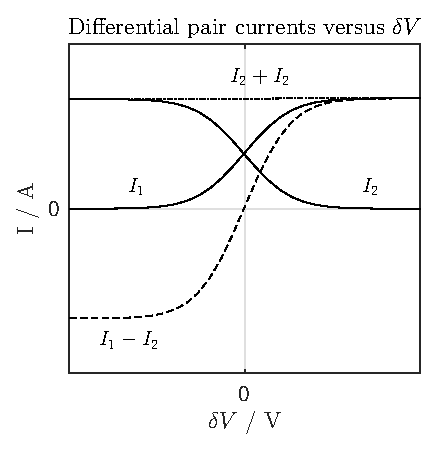
\includegraphics{prelab2.eps}
    \caption{Qualitative graph of the currents observed in the differential pair as \(\delta V\) is swept from negative to positive values.}
    \label{fig:sketch2}
\end{figure}
Fig.~\ref{fig:sketch2} shows a sketch of the currents in the differential pair as a function of \(\delta V\).
\subsection{Simple Current Correlator}
Assuming that \(M_{1in}\), \(M_{2out}\) and \(M_{2in}\), but not \(M_{1out}\) are in saturation, the individual transistor currents are
\begin{align*}
    &I_1 = I_0e^{\frac{\kappa V_1}{U_T}} \\
    &I_2 = I_0e^{\frac{\kappa V_2}{U_T}} \\
    &I_{out} = I_0e^{\frac{\kappa V_1}{U_T}}\left(1-e^{-\frac{V_3}{U_T}}\right) = I_0e^{\frac{\kappa V_2}{U_T}}e^{-\frac{V_3}{U_T}}
\end{align*}
Replacing \(I_0 = I_1w\) where \(w=\frac{W}{L}\) for an individual transistor we have
\begin{align*}
    &\frac{I_{out}}{I_2} = \frac{w_{2out}}{w_{2in}}e^{\frac{-V_3}{U_T}} = r_2e^{\frac{-V_3}{U_T}} \\
    &\frac{I_{out}}{I_1} = \frac{w_{1out}}{w_{1in}}\left(1-e^{\frac{-V_3}{U_T}}\right) = r_1\left(1-e^{\frac{-V_3}{U_T}}\right)
\end{align*}
By substituting \(e^{\frac{-V_3}{U_T}}=\frac{I_{out}}{r_2I_2}\) into the second equation
\begin{align*}
    &\frac{I_{out}}{I_1} = r_1-\frac{r_1I_{out}}{r_2I_2} \\
    &\Updownarrow \\
    &I_{out}\frac{r_1I_1+I_2r_2}{I_1I_2r_2} = r_1 \\
    &\Updownarrow \\
    &I_{out} = \frac{r_1I_1r_2I_2}{r_1I_1+r_2I_2}
\end{align*}
Which is what was to be shown.

\subsection{Current Correlator Continued}
\subsubsection{}
Substituting \(I_1=\frac{I_t}{2}(1+x)\) and \(I_2=\frac{I_t}{2}(1-x)\) into the above equation yields
\begin{align*}
    &I_{out} = \frac{r_1r_2I_t(1+x)(1-x)}{2\left(r_1(1+x)+r_2(1-x)\right)} = \frac{r_1r_2I_t(1-x^2)}{2\left(r_1(1+x)+r_2(1-x)\right)}
\end{align*}
\subsubsection{}
Assuming \(r_1=r_2\equiv r\), the above simplifies to 
\begin{align}
    &I_{out} = \frac{rI_t(1-x^2)}{4}
    \label{eq:q4}
\end{align}
\begin{figure}
    \center
    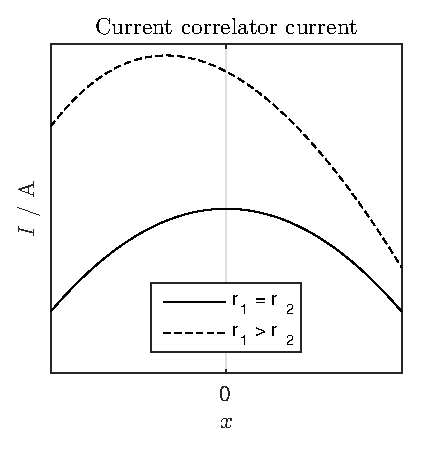
\includegraphics{prelab3.eps}
    \caption{Qualitative sketch of $I_{out}$ for the current correlator using the $I_t$ and $x$ parameters. When \(r_1=r_2\), 
        the output current reaches its maximum when both input currents are equal. When \(r_1 > r_2\) the output current reaches
    its maximum when \(I_1\) is larger, because \(I_1\) dominates the fraction.}
    \label{fig:q3}
\end{figure}
See Fig.~\ref{fig:q3} for a sketch of the output current for the current correlator with \(r_1=r_2\) and \(r_1 > r_2\).
\subsubsection{}
For a differential pair, \(I_b = I_1+I_2\) which is exactly how \(I_t\) was defined, therefore \(I_t=I_b\).
In question 1.h) it was shown that for the differential pair
\begin{align*}
    I_1-I_2 &= I_b \tanh\left(\frac{\kappa(V_1-V_2)}{2U_T}\right)
\end{align*}
And since \(x\equiv \frac{I_1-I_2}{I_t}\) and \(I_t=I_b\) we have
\begin{align}
    x &= \tanh\left(\frac{\kappa(V_1-V_2)}{2U_T}\right)
    \label{eq:q4-2}
\end{align}
\subsection{The Bump-Antibump Circuit}
\subsubsection{}
Substituting \(I_t=I_b-I_{out}\) and Eq.~\ref{eq:q4-2} in Eq.~\ref{eq:q4} yields
\begin{equation*}
    I_{out} = \frac{r}{4}\left(I_b-I_{out}\right)\left(1-\tanh^2\left(\frac{\kappa \delta V}{2U_T}\right)\right)
\end{equation*}
Using the hyperbolic trigonometric identity
\begin{equation*}
    \tanh^2\left(x\right) = \frac{1}{1-\frac{1}{\cosh^2\left(x\right)}}
\end{equation*}
The above can be rewritten
\begin{align*}
    &I_{out} = \frac{r}{4}\left(I_b-I_{out}\right)\frac{1}{\cosh^2\left(\frac{\kappa \delta V}{2U_T}\right)} \\
    &\Updownarrow \\
    &\frac{4}{r}\cosh^2\left(\frac{\kappa \delta V}{2U_T}\right) = \frac{I_b}{I_{out}} - 1 \\
    &\Updownarrow \\
    &I_{out} = \frac{I_b}{1+\frac{4}{r}\cosh^2\left(\frac{\kappa \delta V}{2U_T}\right)}
\end{align*}
\subsubsection{}
See above answer.
\subsubsection{}
If \(V_1=V_2\) then \(\delta V = 0 \rightarrow \cosh^2\left(\frac{\kappa \delta V}{2U_T}\right) = 1\), meaning the the fraction will be 
\begin{equation*}
    \frac{I_{out}}{I_b} = \frac{1}{1+\frac{4}{r}}
\end{equation*}
\subsubsection{}
In the bump-antibump circuit the output \(I_{out}\) reaches its maximum when \(V_1=V_2\), while \(I_1+I_2\) is high when the inputs have dissimilar
values. This can be interpreted as the bump being the soft XNOR operation performed on the inputs, and the anti-bump can be interpreted as the
XOR of the two inputs.
\subsection{Simple Transconductance Amplifier}
The simple transconductance amplifier is a differential pair with a current mirror connected between the input terminals. If all transistors are
operating in saturation, then the current through transistor \(M_3\) will be equal to the curren through \(M_4\). Because the current through \(M_3\)
is set by the gate voltage on transistor \(M_1\), the output current must be equal to the current through \(M_1=M_3=M_4\) minus the current through \(M_2\).
Furthermore, the drain conductance of \(M_2\) must be \(\sim 0\), otherwise the drain voltage of \(M_2\) could simply be raised in order to force the
mirrored current through.
\subsubsection{}
The current through the current mirror is controlled by \(V_1\). In the output open-circuit configuration \(I_{out}\) is zero, and therefore the 
current controlled by \(V_1\) must be forced through transistor \(M_2\). This will cause the drain voltage of \(M_2\) to increase, putting \(M_4\) 
into the ohmic region. The voltage at the common node of the differential pair will also increase to follow \(V_1\) as it increases past \(V_2\).

The output voltage will increase approximately linearly with \(V_1\) while \(V_1 < V_2\). As soon as \(V_1>V_2\), the voltage will shoot up and max out
at \(V_{dd}\) because \(M_2\) is already in saturation and no more current can flow through it, assuming the early voltage is large.
\subsubsection{}
For small differential voltages subthreshold, the transconductance is
\begin{equation*}
    g_m=\frac{I_b\kappa}{2U_T}
\end{equation*}
And in superthreshold 
\begin{equation*}
    g_m=\sqrt{\beta I_b}
\end{equation*}
\subsubsection{}
The transconductance is independent of the output resistance, however the voltage gain is not. With increased output resistance comes increased voltage gain
and therefore the transconductance will be limited in reality because of the supply rail voltage restricting the output voltage.
\subsection{Wide-Range Transconductance Amplifier}
\begin{figure}
    \center
    \begin{circuitikz}\draw
        (0,0) node[nmos] (Mb) {}
        (-1,2) node[nmos] (M2) {}
        (-1,4) node[pmos] (M4) {}
        (-3,4) node[pmos, xscale=-1] (M6) {}
        (-3,-2) node[nmos, xscale=-1] (M7) {}
        (1,2) node[nmos, xscale=-1] (M1) {} 
        (1,4) node[pmos, xscale=-1] (M3) {} 
        (3,4) node[pmos] (M5) {} 
        (3,-2) node[nmos] (M8) {} 
        (Mb.source) to[short] ++(0,-0.0) node[ground] {}
        (Mb.drain) to[short, -*] ++(0,0) 
        (Mb.gate) node[anchor=east] {$V_b$}
        (M2.source) to[short] (M2.source |- Mb.drain) to[short] (Mb.drain)
        (M1.source) to[short] (M1.source |- Mb.drain) to[short] (Mb.drain)
        (M1.drain) to[short, -*] (M3.drain)
        (M2.drain) to[short, -*] (M4.drain)
        (M3.drain) to[short] (M3.gate |- M3.drain) to[short, -*] (M3.gate)
        (M4.drain) to[short] (M4.gate |- M4.drain) to[short, -*] (M4.gate)
        (M3.gate) to[short] (M5.gate)
        (M4.gate) to[short] (M6.gate)
        (M5.source) node[rrail] {}
        (M3.source) node[rrail] {}
        (M4.source) node[rrail] {}
        (M6.source) node[rrail] {}
        (M7.source) node[ground] {}
        (M8.source) node[ground] {}
        (M5.drain) to[short] (M8.drain)
        (M6.drain) to[short] (M7.drain)
        (M7.gate) to[short] (M8.gate)
        (M7.drain) to[short, *-] (M7.gate |- M7.drain) to[short, -*] (M7.gate)
        (M5.drain |- {{(0,2)}}) node {} to[short, *-] ++(1,0) node[anchor=west] {$V_{out}$}
        (M1.gate) node[anchor=west] {$V_1$}
        (M2.gate) node[anchor=east] {$V_2$}
    ;\end{circuitikz}
    \caption{The wide-range transconductance amplifier.}
    \label{fig:wide-transamp}
\end{figure}
Fig.~\ref{fig:wide-transamp} shows a wide-range transconductance amplifier. This version of the transconductance amplifier does not have the same restrictions
on allowable input voltages as the simple transconductance amplifier because the output is completely decoupled from the input. The current mirror connected
to the differential pair will continue to work for large input voltages since only the outer transistors are affected by the final output current.
\subsection{Setup Schematics}
\begin{figure}
    \center
    \begin{circuitikz}[american voltages, american resistors]\draw
        (0,0) node[nmos] (Mb) {}
        (Mb.source) to[short, i=$I_b$] ++(0,-0.1) node[ground] {}
        (Mb.gate) node[anchor=east] {$V_{pot1}$}
        (-1,2) node[nmos] (M1) {}
        (M1.source) to[short, i=$I_1$] (M1.source |- Mb.drain) to[short] (Mb.drain)
        (1,2) node[nmos, xscale=-1] (M2) {}
        (M2.source) to[short, i=$I_2$] (M2.source |- Mb.drain) to[short, -*] (Mb.drain)
        (0,-2.5) node[anchor=north] {$V_{pot2}$} to[short, -*] (0,-2)
        (0,-2) to[R=$10k$] (M2.gate |- {{(0,-2)}}) -- (M2.gate)
        (0,-2) to[R, l_=$10k$] (M1.gate |- {{(0,-2)}}) -- (M1.gate)
        (M1.gate |- {{(0,-4)}}) to[V=K230] (M2.gate |- {{0,-4}})
        (M1.gate |- {{(0,-4)}}) to[short, -*] (M1.gate |- {{(0,-2)}})
        (M2.gate |- {{(0,-4)}}) to[short, -*] (M2.gate |- {{(0,-2)}})
        (M2.drain) node[rrail] {}
        (M1.drain) to[V=K236] ++(0,1) node[rrail] {} 
        (M1.gate) node[anchor=east] {$V_1$}
        (M2.gate) node[anchor=west] {$V_2$}
    ;\end{circuitikz}
    \caption{Experiment 1 setup. The K236 is only used to measure current and is switched between both input current transistors for measurements of both \(I_1\) and \(I_2\).}
    \label{fig:ex1}
\end{figure}
\begin{figure}
    \center
    \begin{circuitikz}[american voltages, american resistors]\draw
        (0,0) node[nmos] (Mb) {}
        (Mb.source) node[ground] {}
        (Mb.drain) to[short, -*] ++(0,0)
        (0,2) node[nmos] (M3) {}
        (0,4) node[nmos,xscale=-1] (M4) {}
        (-2,2) node[nmos] (M1) {}
        (2,2) node[nmos,xscale=-1] (M2) {}
        (M1.source) to[short, i=$I_1$] (M1.source |- Mb.drain) to[short, -*] (Mb.drain)
        (M2.source) to[short, i=$I_2$] (M2.source |- Mb.drain) to[short, -*] (Mb.drain)
        (M3.source) to[short, i=$I_{out}$] (M3.source |- Mb.drain) to[short, -*] (Mb.drain)
        (M3.drain) to[short] (M4.source)
        (M1.gate) to[short] (M3.gate)
        (M2.gate) to[short] (M2.gate -| M4.gate) to[short] (M4.gate)
        (0,-2.5) node[anchor=north] {$V_{pot2}$} to[short, -*] (0,-2)
        (0,-2) to[R=$10k$] (M2.gate |- {{(0,-2)}}) -- (M2.gate)
        (0,-2) to[R, l_=$10k$] (M1.gate |- {{(0,-2)}}) -- (M1.gate)
        (M1.gate |- {{(0,-4)}}) to[V=K230] (M2.gate |- {{0,-4}})
        (M1.gate |- {{(0,-4)}}) to[short, -*] (M1.gate |- {{(0,-2)}})
        (M2.gate |- {{(0,-4)}}) to[short, -*] (M2.gate |- {{(0,-2)}})
        (M2.drain) node[rrail] {}
        (M1.drain) to[V=K236] ++(0,1) node[rrail] {}
        (M1.gate) node[anchor=east] {$V_1$}
        (M2.gate) node[anchor=west] {$V_2$}
        (M4.drain) node[rrail] {}
    ;\end{circuitikz}
    \caption{Experiment 2 setup. The K236 is again only used to measure current and is switched between all three terminals connected to \(V_{dd}\) to measure \(I_1\), \(I_2\) and \(I_{out}\).}
    \label{fig:ex2}
\end{figure}
\begin{figure}
    \center
    \begin{circuitikz}[american voltages, american resistors]\draw
        (0,0) node[nmos] (Mb) {}
        (Mb.source) to[short, i=$I_b$] ++(0,-0.1) node[ground] {}
        (Mb.gate) node[anchor=east] {$V_{pot1}$}
        (-1,2) node[nmos] (M1) {}
        (M1.source) to[short, i=$I_1$] (M1.source |- Mb.drain) to[short] (Mb.drain)
        (1,2) node[nmos, xscale=-1] (M2) {}
        (M2.source) to[short, i=$I_2$] (M2.source |- Mb.drain) to[short, -*] (Mb.drain)
        (-1,4) node[pmos, xscale=-1] (M3) {}
        (1,4) node[pmos] (M4) {}
        (M3.drain) to[short] (M1.drain)
        (M3.drain) to[short, *-] (M3.drain -| M3.gate) to[short, -*] (M3.gate)
        (M4.drain) to[short, -*] (M2.drain)
        (M4.source) node[rrail] {}
        (M3.source) node[rrail] {}
        (M2.drain) to[short, i=$I_{out}$] ++(2,0) node (temp0) {}
        (temp0 |- {{(0,0)}}) node[ground] {} to[V, v_=K236] (temp0)
        (M1.gate) to[short, -*] ++(-1,0) node (temp1) {} to[R] ++(0,2) node[rrail] {}
        (temp1) to[vR, v=$V_{pot2}$] ++(0,-2) node[ground] {}
        (temp1) to[short] ++(-2,0) to[short] ++(0,-4) node (temp2) {} to[V=K230] (M2.gate |- temp2) to[short] (M2.gate)
        (M1.gate) node[anchor=south] {$V_1$}
        (M2.gate) node[anchor=south] {$V_2$}
    ;\end{circuitikz}
    \caption{Experiment 3 and 4 setup. The K236 is used to measure current in experiment 3 and voltage in experiment 4.}
    \label{fig:ex3-4}
\end{figure}
Figures~\ref{fig:ex1}, \ref{fig:ex2} and \ref{fig:ex3-4} show the experimental setups that we will be using.
\end{document}
